
\chapter{Multimodal face-evoked responses}


\section{Overview}

This dataset contains EEG, MEG, functional MRI and structural MRI data on the same subject within the same paradigm, which allows a basic comparison of faces versus scrambled faces.

It can be used to demonstrate, for example, 3D source reconstruction of various electrophysiological measures of face perception, such as the "N170" evoked response (ERP) recorded with EEG, or the analogous "M170" evoked field (ERF) recorded with MEG. These localisations are informed by the anatomy of the brain (from the structural MRI) and possibly by functional activation in the same paradigm (from the functional MRI).

The demonstration below involves localising the N170 using a distributed source method (called an "imaging" solution in SPM) analogous to "weighted minimum L2-norm". The data can also be used to explore further effects, e.g. induced effects (Friston et al, 2006), effects at different latencies, or the effects of adding fMRI constraints on the localisation.

The EEG data were acquired on a 128 channel ActiveTwo system; the MEG data were acquired on a 151 channel CTF Omega system; the sMRI data were acquired using a phased-array headcoil on a Siemens Sonata 1.5T; the fMRI data were acquired using a gradient-echo EPI sequence on the Sonata. The dataset also includes data from a Polhemus digitizer, which are used to coregister the EEG and the MEG data with the structural MRI.

Some related analyses of these data are reported in Henson et al (2005a, 2005b, 2007), Kiebel and Friston (2004) and Friston et al (2006; in press-a).

The analysis below is best done in Matlab7, but all mat files should be in a format readable by Matlab6.5.

\section{Paradigm and Data}

The basic paradigm involves randomised presentation of at least 86 faces and 86 scrambled faces (Figure~\ref{fig_32_1}), based on Phase 1 of a previous study by Henson et al (2003). The scrambled faces were created by 2D Fourier transformation, random phase permutation, inverse transformation and outline-masking of each face. Thus faces and scrambled faces are closely matched for low-level visual properties such as spatial frequency power density. Half the faces were famous, but this factor is collapsed in the current analyses. Each face required a four-way, left-right symmetry judgment (mean RTs over a second; judgments roughly orthogonal to conditions; reasons for this task are explained in Henson et al, 2003). The subject was instructed not to blink while the fixation cross was present on the screen.


\begin{figure}
\begin{center}
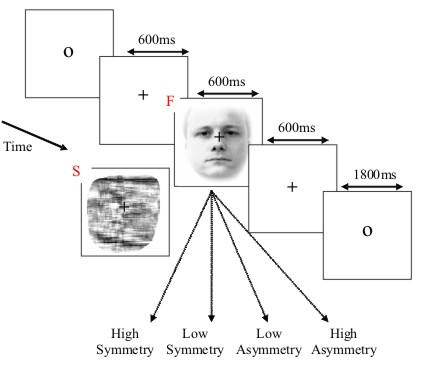
\includegraphics[width=100mm]{multimodal/figures/figure_32_1}
\caption{\em One trial in the experimental paradigm: Trials involved either a Face (F) or Scrambled face (S). \label{fig_32_1}}
\end{center}
\end{figure}

\subsection{Structural MRI}

The T1-weighted structural MRI of a young male was acquired on a 1.5T Siemens Sonata via an MDEFT sequence with resolution $1 x 1 x 1 mm^3$ voxels, using a whole-body coil for RF transmission and an 8-element phased array head coil for signal reception.

The images are in Analyze format in the sMRI sub-directory, consisting of two files:
\begin{verbatim}
	sMRI/sMRI.img
	sMRI/sMRI.hdr
\end{verbatim}
The structural was manually-positioned to match roughly Talairach space, with the origin close to the Anterior Commissure, which produced the associated SPM Matlab file:
\begin{verbatim}
	sMRI/sMRI.mat
\end{verbatim}
The approximate position of 3 fiducials within this MRI space - the nasion, and the left and right peri-aricular points - are stored in the file:
\begin{verbatim}
	sMRI/smri_fids.mat
\end{verbatim}
These were identified manually (based on anatomy) and are used to define the MRI space relative to the EEG and MEG spaces, which need to be coregistered (see below). It doesn't matter that the positions are approximate, because more precise coregistration is done via digitised surfaces of the scalp ("head shape functions") that were created using the Polhemus 3D digitizer.

\subsection{EEG data}

The EEG data were acquired on a 128-channel ActiveTwo system, sampled at 2048 Hz (subsequently downsampled to 200Hz to reduce filesize), plus electrodes on left earlobe, right earlobe, and two bipolar channels to measure HEOG and VEOG. The data were referenced to the average of the left and right earlobes (for consistency with Henson et al, 2003). The 128 scalp channels are named: 32 A (Back), 32 B (Right), 32 C (Front) and 32 D (Left).

The original data were converted into SPM M/EEG format and epoched from -200ms to +600ms post-stimulus (baseline-corrected from -200 to 0ms), ie 161 samples:
\begin{verbatim}
	EEG/e_eeg.mat
	EEG/e_eeg.dat
\end{verbatim}
(using the \verb!bdf_setup.mat! channel template provided with SPM5 in the EEGtemplates sub-directory).
Other details about the data can be examined by typing:
\begin{verbatim}
	D = spm_eeg_ldata
\end{verbatim}
and selecting the \verb!e_meg.mat! file. This will show the contents of the structure "D" that is loaded into the Matlab workspace, the various fields of which can be explored. Note that the data values themselves are memory-mapped from the \verb!e_eeg.dat! file to the field D.data (e.g, D.data(1,2,3) returns the field strength in the first sensor at the second sample point during the third trial).

You will see that there are 344 events (D.Nevents), consisting of 172 faces (event code 1) and 172 scrambled faces (event code 2), which are randomly intermixed (see D.events.code)\footnote{These data were actually concatenated from two separate runs on the same subject (using spm-eeg-merge), which is why there are twice as many events as with the MEG and fMRI data.}. If you type D.channels.name, you will see the order and the names of the channels.

The EEG directory also contains a Polhemus sub-directory with the following files:
\begin{verbatim}
	EEG/Polhemus/eeg_fids.mat
	EEG/Polhemus/eeg_sens_loc.mat
	EEG/Polhemus/eeg_hsf.mat
\end{verbatim}
All files contain matrices, the three columns of which code location in a right-handed 3D space, the axes of which conform to the Talairach space, i.e, the first column is x (left-right), the second is y (anterior-posterior) and the third is z (inferior-superior). The units are mm.

The \verb!eeg_fids.mat! file contains the position of 3 fiducial markers that were placed approximately on the nasion and peri-aricular points and digitised by the Polhemus digitizer. The digitizer was also used to locate the position of each electrode (in the \verb!eeg_sens_loc.mat! file), and to trace out many points along the surface of the subject's scalp and nose (the "head shape function" in the \verb!eeg_hsf.mat! file). Later, we will coregister the fiducial points and the head shape to map the electrode positions in the "Polhemus space" to the "MRI space".

\subsection{MEG data \label{meg}}

The MEG data were acquired on a 151 channel CTF Omega system, using second-order axial gradiometers sampled at 625 Hz (subsequently downsampled to 200Hz to reduce filesize).  The original data were converted into SPM MEEG format and epoched from -200ms to +600ms post-stimulus (i.e, baseline-corrected from -200ms to 0ms), ie 161 samples:
\begin{verbatim}
	MEG/e_meg.mat
	MEG/e_meg.dat
\end{verbatim}
The channel template for these data is also provided:
\begin{verbatim}
	MEG/CTF151_setup.mat
\end{verbatim}
(which may need to be copied to the EEGtemplates sub-directory of your local SPM5 installation directory, if not already there).
The MEG data also contains a Polhemus sub-directory with the following files:
\begin{verbatim}
	MEG/Polhemus/meg_fids.mat
	MEG/Polhemus/meg_sens_loc.mat
	MEG/Polhemus/meg_sens_or.mat
	MEG/Polhemus/meg_hsf.mat
\end{verbatim}
which are analogous to the corresponding MEG files described in the previous section\footnote{These matrices are transformations from the original CTF / Polhemus files - in which x codes anterior-posterior and y codes left-right - i.e, a 90 degree clockwise rotation about the z-axis.}. More specifically, the \verb!meg_fids.mat! contains the position of 3 "locator coils", positioned close to the fiducials\footnote{Unlike the MRI and EEG data, these fiducials were not precisely the nasion and peri-aricular points. However, given that the coregistration of the MEG and MRI data is based mainly on the headshape (see later), this inaccuracy in the MEG fiducials does not matter.}, the locations of which are measured by the CTF machine, and used to define the coordinates (in "CTF space") for the location of the 151 sensors (in the \verb!meg_sens_loc.mat! file) and their (axial gradiometer) orientations (\verb!meg_sens_or.mat!). The same three locator coils were digitised by a Polhemus digitizer outside the MEG machine, together with the head shape, to define the "Polhemus space". Subsequently, the fiducials in the Polhemus space were coregistered with the fiducials in the CTF space, and the resulting rigid-body transformation applied to the Polhemus head shape. Thus the coordinates in all four files above are in alignment in the CTF space, which will subsequently be transformed into the "MRI space".



\subsection{fMRI data}

The fMRI data were acquired using a Trajectory-Based Reconstruction (TBR) gradient-echo EPI sequence (Josephs et al, 2000) on a 1.5T Sonata. There were 32, 3mm slices of 3x3 mm2 pixels, acquired in a sequential descending order with a TR of 2.88s. There are 215 images in the 'Scans' sub-directory (5 initial dummy scans have been removed), each consisting of an Analyze image and header file:
\begin{verbatim}
	fMRI/Scans/fM*.img	
	fMRI/Scans/fM*.hdr
\end{verbatim}
Also provided are the onsets of faces and scrambled faces (in units of scans) in the Matlab file:
\begin{verbatim}
	fMRI/onsets.mat	
\end{verbatim}
and the SPM "Job" files (see Section~\ref{fMRI}):
\begin{verbatim}
	fMRI/realign_job.mat
	fMRI/slicetime_job.mat
	fMRI/smooth_job.mat
	fMRI/stats_job.mat
\end{verbatim}

\section{Getting Started}

You need to start SPM5 and toggle "EEG" as the modality (bottom-right of SPM main window), or start SPM5 with \verb!spm eeg!.
You will also need to 1) copy the MEG template file (\verb!CTF151_setup.mat!) to the EEGtemplates sub-directory within your SPM5 installation directory, if it is not already there (see ~section \ref{meg} above), and 2) ensure this EEGtemplates directory is on your Matlab path.


\section{EEG analysis}

\subsection{Preprocessing the EEG data}

* Change directory to the EEG subdirectory (either in Matlab, or via the "CD" option in the SPM "Utils" menu)

* Press 'Artefacts', select the \verb!e_eeg.mat! file, press 'no' to the 'read own artefact list?' question, 'no' to 'robust average?', 'yes' to 'threshold channels?', and enter 200 for the threshold

This will detect trials in which the signal recorded at any of the channels exceeds 200 microvolts (relative to pre-stimulus baseline). These trials will be marked as artefacts. Most of these artefacts occur on the VEOG channel, and reflect blinks during the critical time window\footnote{Channel-specific thresholds can be used by entering 130 thresholds, one per EEG/EOG channel, with a value of Inf for those channels that you do not want to threshold.}. The procedure will also detect channels in which there are a large number of artefacts (which may reflect problems specific to those electrodes, allowing them to be removed from subsequent analyses).

In this case, the Matlab window will show:
\begin{verbatim}
	There isn't a bad channel.
	45 rejected trials: [5 38 76 82 83 86 87 88 89 90 92 93 94 96 98 99
    100 101 104 105 106 107 108 112 117 118 119 120 122 124 126 130 137
    139 159 173 221 266 268 279 281 292 293 298 326]
\end{verbatim}
(leaving 299 valid trials). A new file will also be created, \verb!ae_eeg.mat!(in which these artefacts are coded in the fields D.events.reject and D.channels.thresholded).

At this point, you may want to look at the data. Press "Display: M/EEG", and select the \verb!ae_eeg.mat! file. After a short delay, the Graphics window should show the mean ERP (for trial 1) at each of the 130 channels (as in Figure~\ref{fig_32_2}). You can click on one of the channels (e.g, VEOG, on the top right of the display) to get a new window with the data for that channel expanded. You can alter the scaling or trial number using the sliders on the bottom of the Graphics window, or select a subset of channels to display by pressing the 'Channels' button.

\begin{figure}
\begin{center}
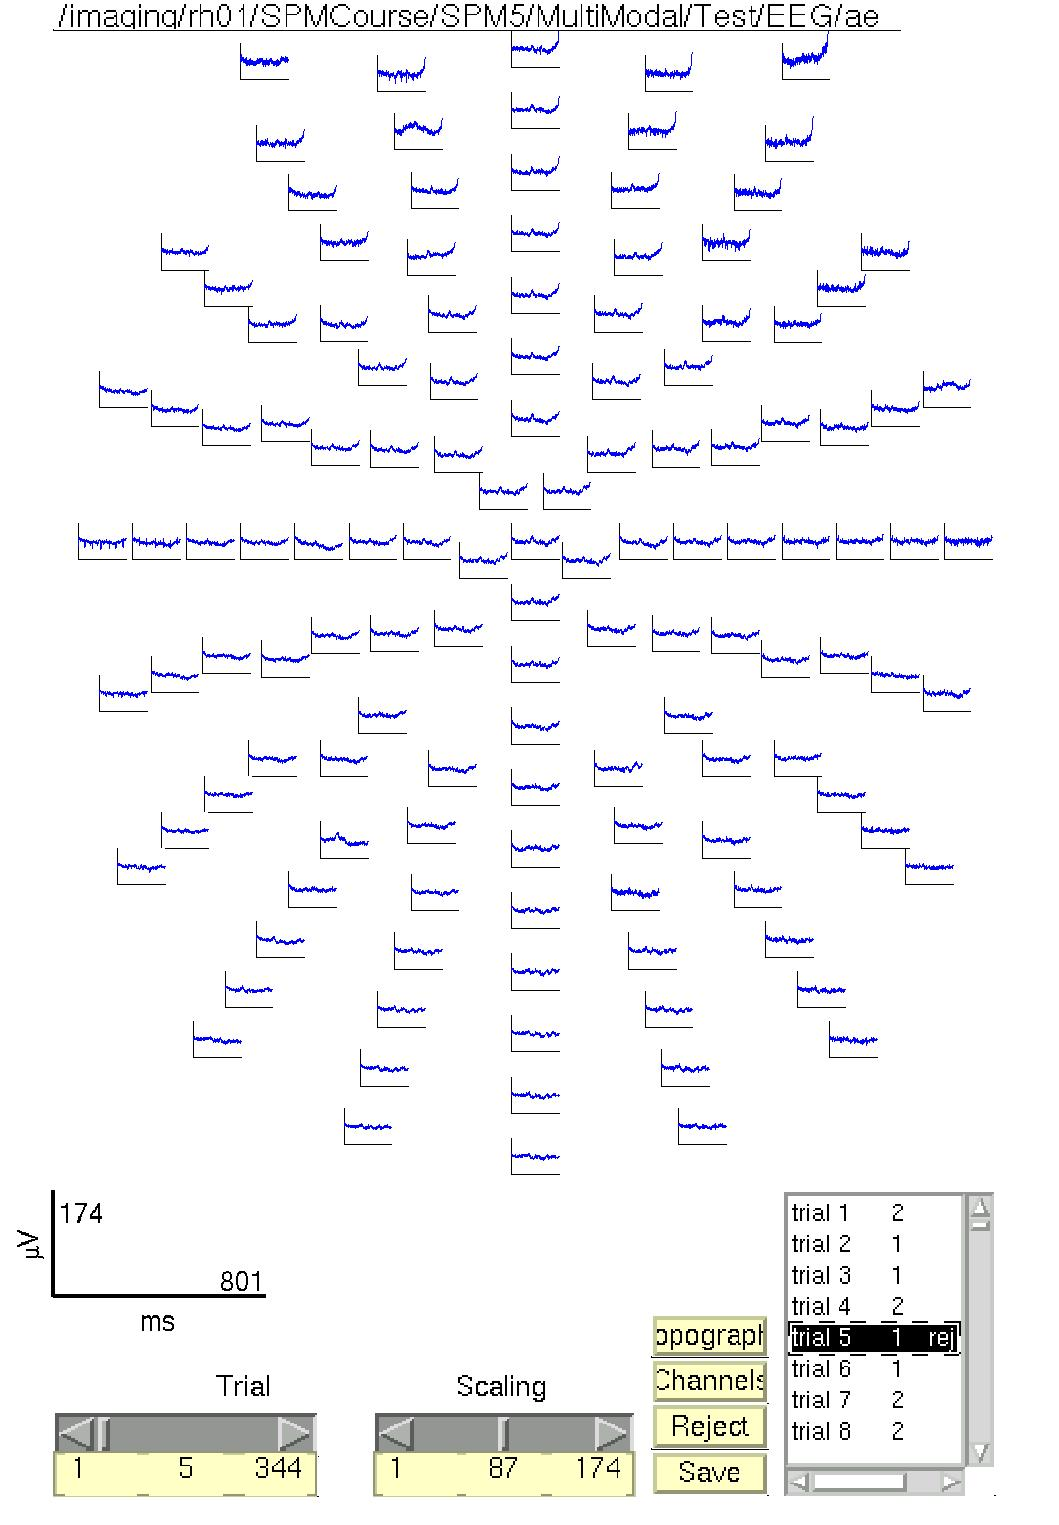
\includegraphics[width=100mm]{multimodal/figures/figure_32_2}
\caption{\em  SPM Display window for trial 5 for all 128 EEG plus 2 EOG channels (top left and top right) in ae-eeg.mat. Trial 5 is marked as an artefact because the VEOG channel (top right) exceeds the user-specified threshold of 200uV, most likely reflecting the onset of a blink towards the end of the epoch. \label{fig_32_2}}
\end{center}
\end{figure}



\subsection{Basic ERPs}

* Press the 'Averaging' button and select the \verb!ae_eeg.mat! file. After a few moments, the matlab window will echo:

	\verb!ae_eeg.mat!: Number of replications per contrast:
	average 1: 151 trials, average 2: 148 trials

	(artefact trials are excluded from averaging) and a new file will be created in 	the MEG directory called \verb!mae_eeg.mat! ("m" for "mean").

* Press the 'Filtering' button, select the \verb!mae_eeg.mat! file, select 'lowpass', and enter 40 (Hz) as the cutoff. This smooths the data to 40Hz, producing the file \verb!fmae_eeg.mat! (using zero-phase-shift forward and reverse digital filtering with a 5th-order Butterworth filter)\footnote{Note that (lowpass) filtering short epochs like this is not necessarily a good idea, since ringing or "end-effects" can result at the start and end of the epoch. Filtering is normally better performed on continuous data (or longer epochs). The filtering performed here is simply to demonstrate the option and for display purposes (though the averaging process also tends to act like a lowpass filter anyway).}.

You can display the mean ERPs using the "Display: M/EEG" menu option again. Once you have done so, press the "channels" button in the Graphics window, then "Deselect all", and then click only, eg channels 'a1', 'd7', 'a12', 'b9' and 'c7'. (You can save these selections as a file, and use this file to display only a subset of channels in future). After pressing "ok", you will now only see these 5 channels (which will also make the display much faster!). Once you hold SHIFT and select trial-type 2, you should see something like Figure~\ref{fig_32_3}.

\begin{figure}
\begin{center}
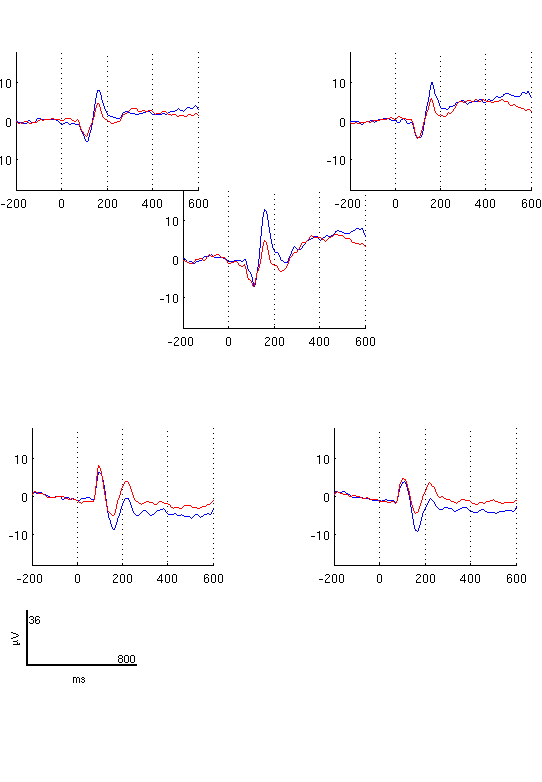
\includegraphics[width=100mm]{multimodal/figures/figure_32_3}
\caption{\em SPM Display window for smoothed, average ERPs for faces (blue) and scrambled faces (red) for 5 selected channels in fmae-eeg.mat. \label{fig_32_3}}
\end{center}
\end{figure}

* Select "Contrast" from the "Other..." pulldown menu on the SPM window (or type \verb!spm_eeg_weight_epochs! in the Matlab window). This function creates linear contrasts of ERPs/ERFs. Select the \verb!fmae_eeg.mat! file, and enter $[1 -1; 1/2 1/2]$ as the contrast matrix. Press "no" to the question "weight by num replications". This will create new file \verb!mfmae_eeg.mat!, in which the first trial-type is now the differential ERP between faces and scrambled faces, and the second trial-type is the average ERP for faces and scambled faces.

To look at the differential ERP, again press 'Display: M/EEG', and select the \verb!mfmae_eeg.mat! file. After a short delay, the Graphics window should show the ERP for each channel (for trial-type 1). Hold SHIFT and select trial-type 2 to see both conditions superimposed. Then click on one of the channels (e.g, 'B9' on the bottom right of the display) to get a new window with the data for that channel expanded, as in Figure~\ref{fig_32_4}.

\begin{figure}
\begin{center}
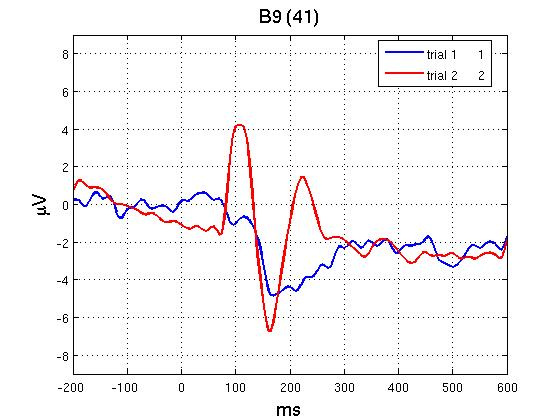
\includegraphics[width=100mm]{multimodal/figures/figure_32_4}
\caption{\em  Average (red) and differential (blue) ERPs for faces and scrambled faces at channel B9 in mfmae-eeg.mat. \label{fig_32_4}}
\end{center}
\end{figure}

The red line shows the average ERP evoked by faces and scrambled faces (at this occipitotemporal channel). A P1 and N1 are clearly seen. The blue line shows the differential ERP between faces and scrambled faces. This is approx zero around the P1 latency, but negative around the N1 latency. The latter likely corresponds to the "N170" (Henson et al, 2003). We will try to localise the cortical sources of the P1 and N170 in Section~\ref{3D}.

To see the topography of the differential ERP, press the "topography" button in the main graphics window, enter 165ms for the latency, and select "3D", to produce Figure~\ref{fig_32_5}. Choose the rotate3D cursor to surf.

\begin{figure}
\begin{center}
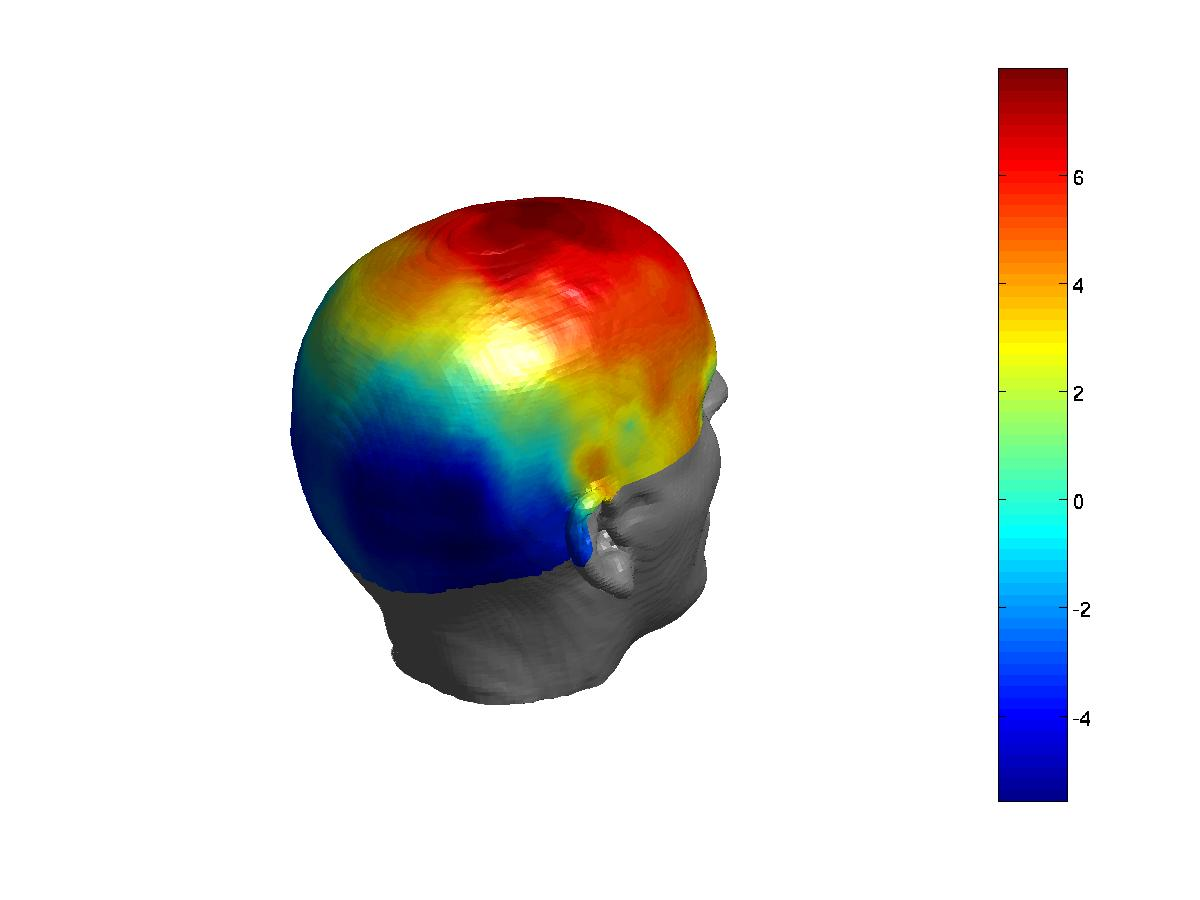
\includegraphics[width=100mm]{multimodal/figures/figure_32_5}
\caption{\em 3D topography for faces minus scrambled faces at 165ms. \label{fig_32_5}}
\end{center}
\end{figure}


\subsection{3D SPMs (Sensor Maps over Time) \label{3DSPM}}

One novel feature of SPM is the ability to use Random Field Theory to correct for multiple statistical comparisons across N-dimensional spaces. For example, a 2D space representing the scalp data can be constructed by flattening the sensor locations and interpolating between them to create an image of MxM pixels (when M is user-specified, eg M=32). This would allow one to identify locations where, for example, the ERP amplitude in two conditions at a given timepoint differed reliably across subjects, having corrected for the multiple t-tests performed across pixels. That correction uses Random Field Theory, which takes into account the spatial correlation across pixels (i.e, that the tests are not independent). This kind of analysis is described earlier in the SPM manual, where a 1st-level design is used to create the images for a given weighting across timepoints of an ERP/ERF, and a 2nd-level design can then be used to test these images across subjects.

Here, we will consider a 3D example, where the third dimension is time, and test across trials within the single subject. We first create a 3D image for each trial of the two types, with dimensions MxMxS, where S=161 is the number of samples. We then take these images into an unpaired t-test across trials (in a 2nd-level model) to compare faces versus scrambled faces. We can then use classical SPM to identify locations in space and time in which a reliable difference occurs, correcting across the multiple comparisons entailed. This would be appropriate if, for example, we had no a priori knowledge where or when the difference between faces and scrambled faces would emerge\footnote{Note that the 2D location in sensor space for EEG will depend on the choice of reference channel.}.

* Select the "mat-2-3Dimage" option in the "Other..." menu in the Matlab window, and select the \verb!ae_eeg.mat! file. You will then be prompted for "output image dimensions", for which you can accept the default of 32 (leading to a 32x32 pixel space), and a pixel dimension, which you can change to 5 (this is rather arbitrary, but will make the images easier to view). It will then ask whether you want to interpolate or mask out bad channels, for which you can select interpolate (though it will make no difference here because there are no bad channels).

This will take some time as it writes out an image for each trial (except rejected trials), in a new directory called \verb!ae_eeg!, which will itself contain two subdirectories, one for each trialtype. In each trialtype subdirectory there will be image and header files for each non-rejected trial of that type, e.g, trial02.img/hdr. You can press "Display: images" to view one of these images - it will have dimensions 32x32x161(x1), with the origin set at [16  16  40] (where 40 samples is 0ms), as in Figure~\ref{fig_32_6}.


\begin{figure}
\begin{center}
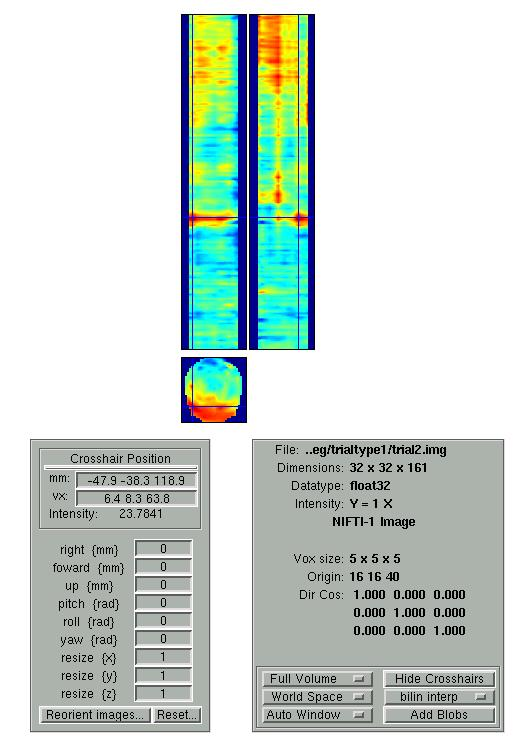
\includegraphics[width=100mm]{multimodal/figures/figure_32_6}
\caption{\em  3D image for trial 2 of ae-eeg.mat. The bottom image is a square 2D x-y space interpolated from the flattened electrode locations (at one point in time). The two top images are sections through x and y respectively, now expressed over time (vertical (z) dimension). (Colormap changed to 'jet').\label{fig_32_6}}
\end{center}
\end{figure}


To perform statistics on these images, first create a new directory, eg. mkdir XYTstats.

* Then press the "specify 2nd level" button,  select "two-sample t-test" (unpaired t-test), and define the images for "group 1" as all those in the subdirectory "trialtype1" (using right mouse, and "select all") and the images for "group 2" as all those in the subdirectory "trialtype2". Finally, specify the new XYTstats directory as the output directory, and press "run"\footnote{Note that we can use the default "nonsphericity" selections, i.e, that the two trial-types may have different variances, but are uncorrelated.}.



This will produce the design matrix for a two-sample t-test.

* Then press "Estimate", and when it has finished, press "Results" and define a new F-contrast as [1 -1] (for help with these basic SPM functions, see eg. chapter 26). Keep the default contrast options, but threshold at $p<.05$ FWE corrected for the whole "image". Then press "volume", and the Graphics window should now look like that in Figure~\ref{fig_32_7} (ignore the outline of the brain in the MIP!).

This will reveal "regions" within the 2D sensor space and within the -200ms to 600ms epoch in which faces and scrambled faces differ reliably, having corrected for multiple F-tests across pixels/time. There are a number of such regions, but we will concentrate on the first two (largest ones), with cluster maxima of  [25 -55 200] and [10 5 160]. An F-test was used because the sign of the difference reflects the polarity of the ERP difference, which is not of primary interest (and depends on the choice of reference; see footnote 6). Indeed, if you plot the contrast of interest from the cluster maxima, you will see that the difference is negative for the first cluster (which is located posteriorly) but positive for the second cluster (which is more central, close to Cz). This is consistent with the polarity of the differences in Figure~\ref{fig_32_3}\footnote{With a reference similar to the current earlobes, the former likely corresponds to the "N170", while the latter likely corresponds to the "VPP" (though we have no evidence here for a dissociation between them).}.

If one had more constrained a priori knowledge about where and when the N170 would appear, one could perform an SVC based on, for example, a box around posterior channels and between 150 and 200ms poststimulus.

\begin{figure}
\begin{center}
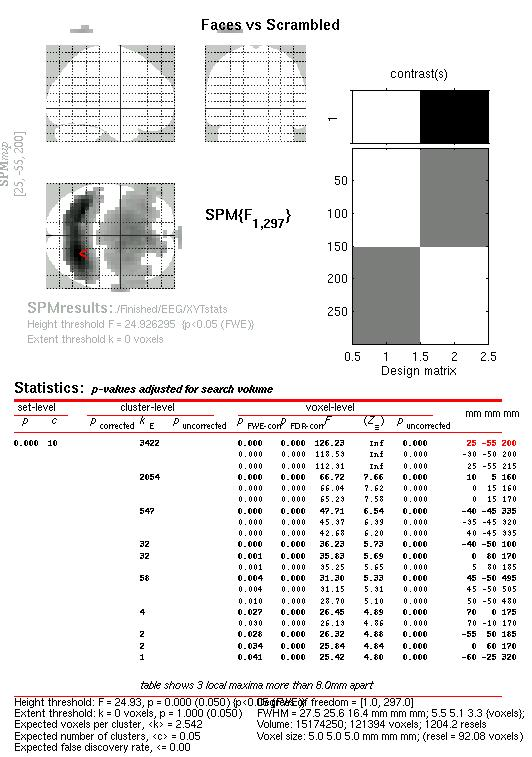
\includegraphics[width=100mm]{multimodal/figures/figure_32_7}
\caption{\em 3D sensor-time SPM{F} at $p<.05$ FWE corrected for the amplitude difference between face and scrambled face trials. Note that the brain outline in the MIP should be ignored. The x, y coordinates refer to arbitrary units in the 32x32 electrode plane (origin = [16 16]); the z coordinate refers to peristimulus time in ms (to the nearest sampling of 5ms). \label{fig_32_7}}
\end{center}
\end{figure}

\subsection{3D "imaging" reconstruction \label{3D}}

Here we will demonstrate a distributed source reconstruction of the N170 differential evoked response between faces and scrambled faces, using a grey-matter mesh extracted from the subject's MRI, and an L2-norm method in which multiple constraints on the solution can be imposed (Phillips et al, 2002; Mattout et al, 2005; Henson et al, 2007; Friston et al, in press-a).

* Press the '3D source reconstruction' button, and press the "load" button at the top of the new window. Select the \verb!mfmae_eeg.mat! file and type a label (eg "N170") for this analysis\footnote{Note that no new M/EEG files are created during each stage of the 3D reconstruction; rather, each step involves updating of the cell-array field D.inv, which will have one entry per analysis performed on that dataset (e.g, D.inv\{1\} in this case).}.

* Press the 'MRI' button, select the smri.img file within the sMRI sub-directory, press the "Imaging" button, and select 3000 for the number of vertices in the mesh...

The "imaging" option corresponds to a distributed source localisation, where current sources are estimated at a large number of fixed points (3000 here) within a cortical mesh, rather than approximated by a small number of equivalent dipoles (the ECD option). The imaging or distributed approach is better suited for group analyses and probably for later components; the ECD approach may be better suited for very early sensory components (when only small parts of the brain are active), or for DCM models of a small number of regions (Kiebel et al, 2006).

This will take some time while the MRI is segmented (and normalisation parameters determined). This will create the usual files, i.e, c1/c2/c3smri.img/hdr, for grey/white/CSF respectively, msmri.img/hdr for the attentuation-corrected image, and the normalisation and inverse normalisation parameters (\verb!mri_vbm_sn_1.mat! and \verb!smri_vbm_inv_sn_1.mat! respectively) in the sMRI directory (see Chapter 5 for further details).

This process will also create binary images of the cortex, inner skull surface and scalp, which are then used to create meshes (of 2002 vertices) for these surfaces, stored in the following files:
\begin{verbatim}
		sMRI/smri_cortex.img
		sMRI/smri_iskull.img
		sMRI/smri_scalp.img
\end{verbatim}
When meshing has finished, the cortex (blue), inner skull (red) and scalp (orange) meshes will also be shown in the Graphics window. The field D.inv\{1\}.mesh field will be updated in matlab. Press "save" in top right of window to update the corresponding mat file on disk.

Note that the cortical mesh (and the distances within the mesh) are not created directly from the segmented MRI (like the skull and scalp meshes), but rather are determined from a template cortical mesh in MNI space via inverse spatial normalisation (Mattout et al, in press).

* Press the 'Co-register' button, respond "no" to the 'Read Polhemus?' question (which is if you want to read in a Polhemus file directly), and then select the following files in response to each prompt (pressing "yes" to the 'Use headshape file' prompt):
\begin{verbatim}
  		EEG/Polhemus/eeg_sens_loc.mat
   		EEG/Polhemus/eeg_fids.mat
   		EEG/Polhemus/eeg_hsf.mat
   		sMRI/smri_fids.mat
\end{verbatim}
This stage coregisters the EEG sensor positions with the structural MRI and cortical mesh, via an approximate matching of the fiducials in the two spaces, followed by a more accurate surface-matching routine that fits the head-shape function (measured by Polhemus) to the scalp that was created in the previous meshing stage via segmentation of the MRI.

When coregistration has finished, the field D.inv\{1\}.datareg will be updated in matlab. Press "save" in top right of window to update the corresponding mat file on disk. Finally, a figure like that in Figure~\ref{fig_32_8} will also be produced, which you can rotate with the mouse (using the Rotate3D Matlab Menu option) to check all sensors.


\begin{figure}
\begin{center}
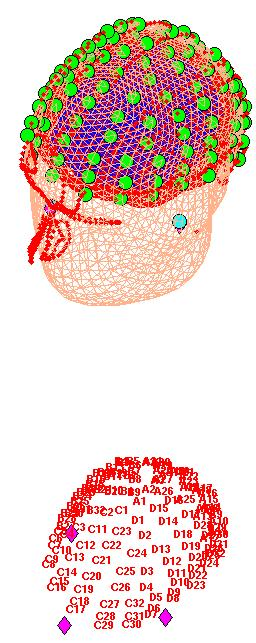
\includegraphics[width=70mm]{multimodal/figures/figure_32_8}
\caption{\em  Graphical output of Co-registration of EEG data, showing (upper panel) cortex (blue), inner skull (red) and scalp (black) meshes, electrode locations (green), MRI/Polhemus fiducials (cyan/magneta), and headshape (red dots).\label{fig_32_8}}
\end{center}
\end{figure}

\noindent * Press 'Forward Model', and select "3 {Berg}".

This will create a forward model (lead field matrix) based on a three sphere model (using a subset of BrainStorm functions, packaged with SPM~\footnote{Brainstorm is available from http://neuroimage.usc.edu/ResearchMEGEEGBrainStorm.html}). The Matlab window will output:
\begin{verbatim}
	Scalp best fitting sphere computed (in 11 iterations)
	Centre = [0.0001 -0.0218 0.0027] (Radius = 0.0774)
	Computing EEG "BERG" Parameters. . .
	Computing EEG "BERG" Parameters -> DONE

	Computing the Image Gain Matrices. . .
	Foward model complete - thank you
 \end{verbatim}

and a picture of the best-fitting sphere to the inner skull surface will be shown in the Graphics window (this defines the centre of the concentric spheres). The leadfield matrix (with source orientations fixed as normal to the cortical surface) is stored in the file:
\begin{verbatim}
	smri_SPMgainmatrix_1.mat
\end{verbatim}
(The file \verb!smri_SPMgainmatxyz_1.mat! stores a version with three orthogonal orientations per source location).

* Press 'Invert', select "Classical" (i.e, a distributed solution rather than DCM; Kiebel et al, 2006), select "yes" to include all conditions (i.e, both the differential and common effects of faces and scrambled faces), press "MSP" for the type of inversion, and then "Standard".

MSP stands for "Multiple Sparse Priors", and has been shown to be superior to standard minimum norm (the alternative MNM option) or a maximal smoothness solution (like LORETA; the COH option) - see Friston et al (in press-a). Note that by default, MSP uses a "Greedy Search" (Friston et al, in press-b), though the standard ReML (as used in Friston et al, in press-a) can be selected as a hidden option.

The "Standard" option uses default values for the MSP approach (to customise some of these parameters, press "Customise" instead).

* Press "save" to save the results. You can now explore the results via the 3D reconstruction window. If you type 165 into the box in the bottom right (corresponding to the time in ms) and press "mip", you should see an output like in~\ref{fig_32_9}. This fit explains approx 97\% of the data.

Note the hot-spots in the fusiform. The timecourses come from the peak voxel. The red line shows the condition currently being shown (corresponding to the "Condition 1" toggle bar in the reconstruction window); the grey line(s) will show all other conditions. Condition 1 is the differential evoked responses for faces vs scrambled; if you press the "condition 1" toggle, it will change to Condition 2 (average evoked response for faces and scrambled faces), then press "mip" again and the display will update (note the colours of the lines have now reversed from before, with red now corresponding to average ERP).

If you toggle back to condition 1 and press "movie", you will see the changes in the source strengths for the differential response over peristimulus time (from the limits 0 to 300ms currently chosen by default).

If you press "render" you can get a very neat graphical interface to explore the data (the buttons are fairly self-explanatory). However, we will concentrate on how one might perform statistics (eg with more subjects in a group analysis).


\begin{figure}
\begin{center}
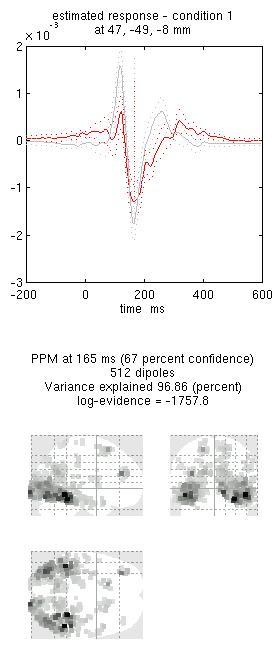
\includegraphics[width=100mm]{multimodal/figures/figure_32_9}
\caption{\em Graphical output of an MSP estimation of the differential ERP between faces and scrambled faces at 165ms. \label{fig_32_9}}
\end{center}
\end{figure}

\noindent * Press the "Window" button in the reconstruction window, enter "150 200" as the timewindow of interest and keep "0" as the frequency band of interest (0 means all frequencies). The Graphics window will then show the mean activity for this time/frequency contrast (and the contrast itself; note additional use of a Hanning window).

\noindent * If you then press "Image", press "12" for the smoothing kernel, and SPM will write 3D Nifti images corresponding to the above contrast for each condition:
\begin{verbatim}
	w_mfmae_eeg_1_1.nii
	w_mfmae_eeg_1_2.nii
	sw_mfmae_eeg_1_1.nii
	sw_mfmae_eeg_1_2.nii
\end{verbatim}
Note that the first two images are unsmoothed (but normalised); the latter two are smoothed by a 12mm isotropic Gaussian kernel. The last number in the file name refers to the condition number; the penultimate number refers to the reconstruction number (ie the number in red in the reconstruction window, i.e, D.val, here 1).

The smoothed results for Condition 1 (i.e, the differential evoked response for faces vs scrambled faces) will also be displayed in the Graphics window, together with the normalised structural. Note that the solution image is in MNI (normalised) space, because the use of a canonical mesh provides us with a mapping between the cortex mesh in native space and the corresponding MNI space.

You can also of course view the image with the normal SPM "Display:image" option, and locate the coordinates of the "hotspots" in MNI space. Note that these images contain RMS (unsigned) source estimates (see Henson et al, 2007).

You could also explore the other inversion options, like COH and MNM, which you will note give more superficial solutions (a known problem with standard minimum norm). To do this quickly (without repeating the MRI segmentation, coregistration and forward modelling), press the "new" button in the reconstruction window, which by default will copy these parts from the previous reconstruction.


\section{MEG analysis}

\subsection{Preprocessing the MEG data}

* Change directory to the MEG subdirectory (either in Matlab, or via the "CD" option in the SPM "Utils" menu)

* Press 'Artefacts', select the \verb!e_meg.mat! file, press 'no' to the 'read own artefact list?' question, but 'yes' to 'robust average?' and select the default 'offset weighting function' (3) and default FWHM residual smoothing (20), and 'no' to 'threshold channels?'

This will take a while. The new file produced, \verb!ae_meg.mat!, will contain the same data, but a new field of "D.weights" will be created. These weights will be applied during the next step of averaging (see Kilner et al, in prep.):

* Press the 'Averaging' button and select the \verb!ae_meg.mat! file. After a few moments, the matlab window will echo:
\begin{verbatim}
	e_meg.mat: Number of replications per contrast:
	average 1: 86 trials, average 2: 86 trials
\end{verbatim}
	and a new file will be created in the MEG directory called \verb!mae_meg.mat! 	 ("m" for "mean")

* Press the 'Filtering' button, select the \verb!mae_eeg.mat! file, select 'lowpass', and enter 40 (Hz) as the cutoff. This smooths the data to 40Hz, producing the file \verb!fmae_eeg.mat! (see again footnote 5 about filtering).

As before, you can display these data by "Display: M/EEG" and selecting the \verb!fmae_eeg.mat!. Hold SHIFT and select trial-type 2 with the mouse in the bottom right of the window to see both conditions superimposed (as Figure~\ref{fig_32_10}).

\begin{figure}
\begin{center}
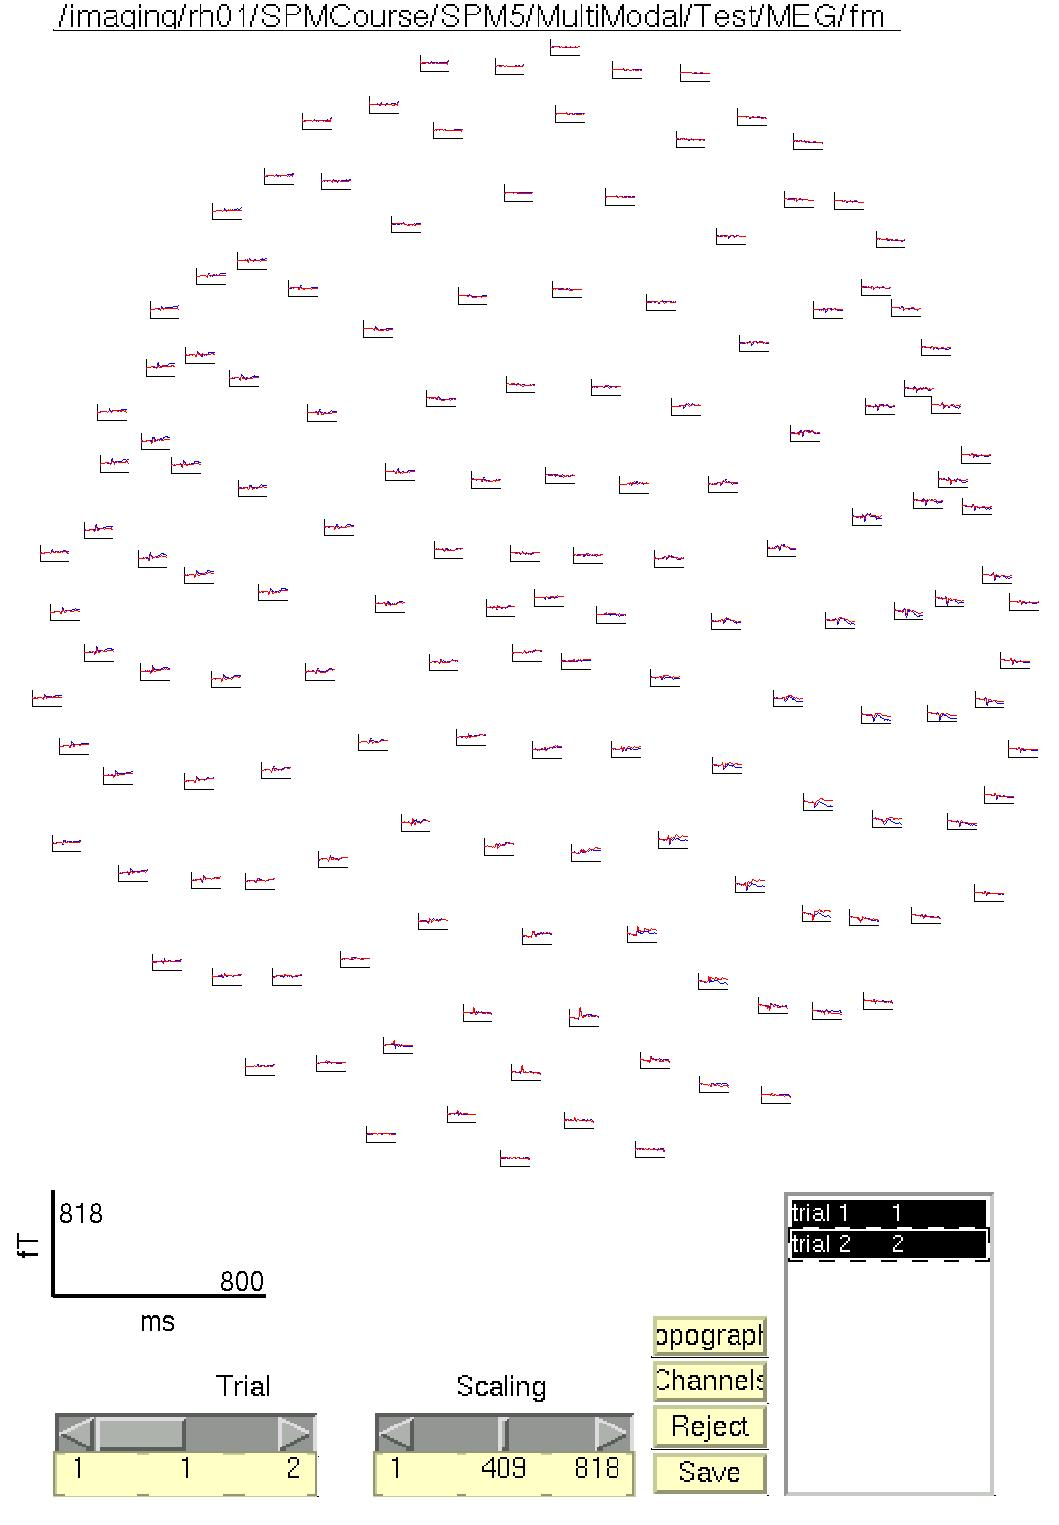
\includegraphics[width=100mm]{multimodal/figures/figure_32_10}
\caption{\em SPM Display window for mean, smoothed ERF (fmae-meg.mat) for all 151 MEG channels. \label{fig_32_10}}
\end{center}
\end{figure}

You can also press this 'Channels' button and in the new window, "deselect" all the channels, then select MRT24 and MLT24 (e.g, from the channel names on the right), and press 'ok'. (It will help if you save these selections as a file, which can be used later to display only a subset of channels). You will now only see these two channels in the SPM Graphics Window, which clearly show a difference between faces (trial-type 1, in blue) and scrambled faces (trial-type 2, in red) around approximately 170ms (the "M170"; Figure~\ref{fig_32_11}). The sign of this difference is reversed across left and right hemispheres, as is common for the axial components of the magnetic fields from tangential current sources.


\begin{figure}
\begin{center}
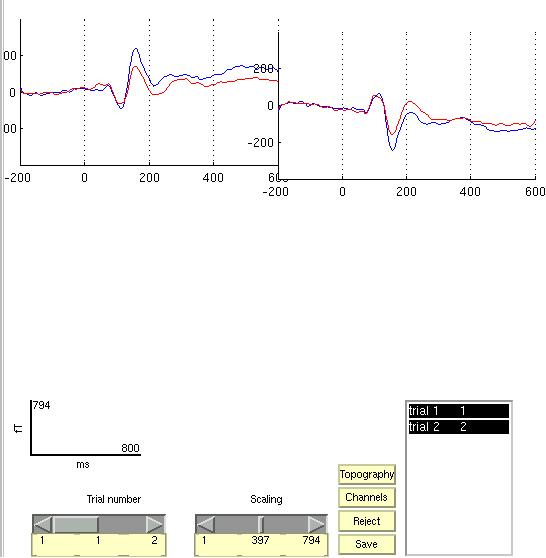
\includegraphics[width=100mm]{multimodal/figures/figure_32_11}
\caption{\em Two selected MEG channels (MLT24 and MRT24). \label{fig_32_11}}
\end{center}
\end{figure}

* Select "Contrast" from the "Other..." pulldown menu on the SPM window (or type \verb!spm_eeg_weight_epochs! in the Matlab window). This function creates linear contrasts of ERPs/ERFs. Select the \verb!fmae_meg.mat! file, and enter [1 -1; 1/2 1/2]as the contrasts. This will create new file \verb!mfmae_meg.mat!, in which the first trial-type is now the differential ERF between faces and scrambled faces, and the second trial-type is the average ERF.

If you want to see the 2D topography of the differential ERF between faces and scrambled faces, you can Display the new file \verb!mfmae_eeg.mat!, select trial-type 1, press "Topography" and in the new window, select "2D" and 165ms as the timepoint (Figure~\ref{fig_32_12}). This will show a bilinear interpolation of the difference across the 151 channels.

You can move the slider left and right to see the development of the M170 over time.

\begin{figure}
\begin{center}
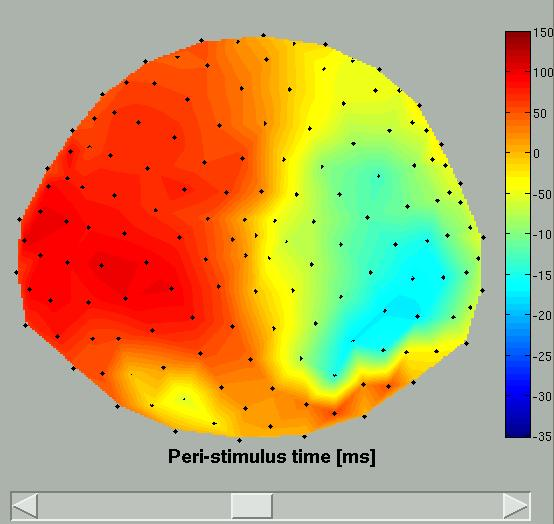
\includegraphics[width=100mm]{multimodal/figures/figure_32_12}
\caption{\em 2D topography of the ERF of faces minus scrambled faces at 165ms\label{fig_32_12}}
\end{center}
\end{figure}

\subsection{Time-Frequency Analysis}

SPM uses Morlet wavelets to perform time-frequency analyses.

* Select the 'time-frequency' option under the 'Other' pull-down menu, and select the \verb!ae_meg.mat! file. SPM will then prompt you for the frequencies you wish to analyse, for which you can type [5:40] (Hz). To the question "remove baseline", press "no" (because for frequencies as low as 5Hz, one would need a longer pre-stimulus baseline, to avoid edge-effects\footnote{For example, for 5Hz, one would need at least N/2 x 1000ms/5, where N is the order of the Morlet wavelets (i.e, number of cycles per Gaussian window), e.g, 600ms for a 6th-order wavelet.}). Later, we will compare two trial-types directly, and hence any pre-stimulus differences will become apparent. Change the default Morlet wavelet order (N) from 7 to 5. This factor effectively trades off frequency vs time resolution, with a lower order giving higher temporal resolution. You will then be prompted to select channels, for which you can highlight and delete the default option of all channels, and type just 66 (which corresponds to channel 'MLT34', as can be confirmed by typing D.channels.names in the Matlab window)\footnote{You can of course obtain time-frequency plots for every channel, but it will take much longer (and result in a large file).}.

This will produce two new files, \verb!t1_e_eeg.mat! and  \verb!t2_e_eeg.mat!. The former contains the power at each frequency, time and channel; the latter contains the corresponding phase angles.

* Press the 'Averaging' button and select the \verb!t1_e_meg.mat! file. After a few moments, the matlab window will echo:
\begin{verbatim}
	e_meg.mat: Number of replications per contrast:
	average 1: 86 trials, average 2: 86 trials
\end{verbatim}
	and a new file will be created in the MEG directory called \verb!mt1_e_meg.mat!.

This contains the power spectrum averaged over all trials, and will include both "evoked" and "induced" power. Induced power is (high-frequency) power that is not phase-locked to the stimulus onset, which is therefore removed when averaging the amplitude of responses across trials (i.e, would be absent from a time-frequency analysis of the \verb!mae_eeg.mat! file).

The power spectra for each trial-type can be displayed using the usual Display button and selecting the \verb!mt1_e_eeg.mat! file. This will produce a plot of power as a function of frequency (y-axis) and time (x-axis) for Channel MLT34. If you use the "trial" slider to switch between trial(types) 1 and 2, you will see the greater power around 150ms and 10Hz for faces than scrambled faces (click on one channel to get scales for the axes, as in Figure~\ref{fig_32_13}). This corresponds to the M170 again.

\begin{figure}
\begin{center}
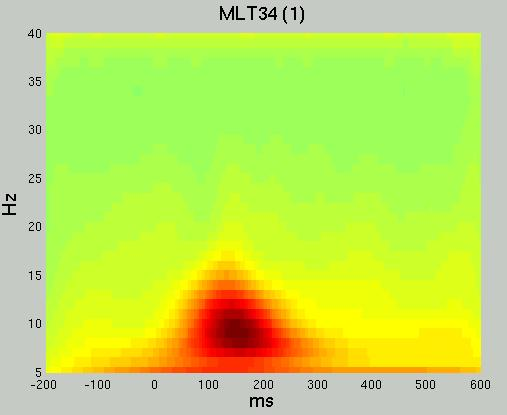
\includegraphics[width=60mm]{multimodal/figures/figure_32_13_L}
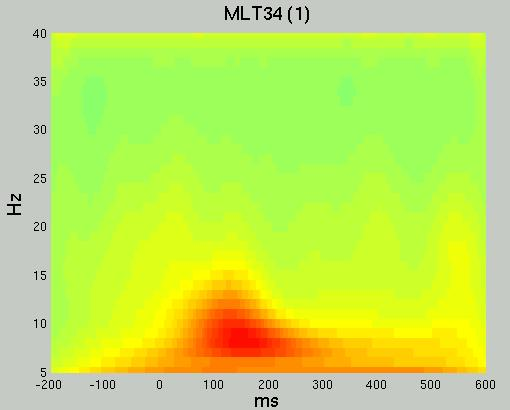
\includegraphics[width=60mm]{multimodal/figures/figure_32_13_R}
\caption{\em  Total power spectra for faces (left) and scrambled faces (right) for channel MLT34\label{fig_32_13}}
\end{center}
\end{figure}

We can also look at evidence of phase-locking of ongoing oscillatory activity by averaging the phase angle information. This time, we do not take the straight (arithmetric) mean, since the data are phase angles, and this average is not particularly meaningful. Instead we calculate their vector mean (when converting the angles to
vectors in Argand space), which corresponds to a "Phase-Locking Value" (PLV) which lies between 0 (no phase-locking across trials) to 1 (perfect phase-locking).

* Press the 'Averaging' button and select the \verb!t2_e_meg.mat! file. This time you will be prompted for either a straight or a vector average, for which you should select "vector". The matlab window will echo:
\begin{verbatim}
	e_meg.mat: Number of replications per contrast:
	average 1: 86 trials, average 2: 86 trials
\end{verbatim}
	and a new file will be created in the MEG directory called \verb!mt2_e_meg.mat!.

If you now display the file \verb!mt2_e_eeg.mat! file, you will see PLV as a function of frequency (y-axis) and time (x-axis) for Channel MLT34. Again, if you use the "trial" slider to switch between trial(types) 1 and 2, you will see greater phase-locking around 10Hz and 100ms for faces than scrambled faces, as in Figure~\ref{fig_32_14}. Together with the above power analysis, these data suggest that the M170 includes an increase both in power and in phase-locking of ongoing oscillatory activity in the alpha range (Henson et al, 2005b).


\begin{figure}
\begin{center}
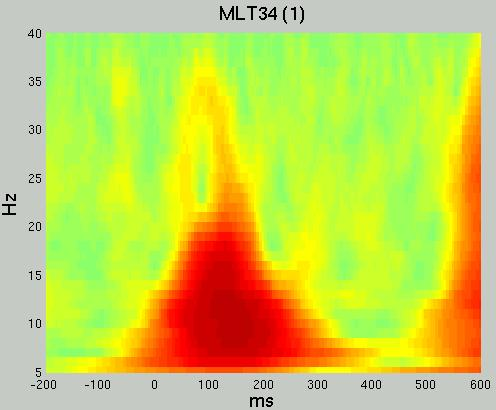
\includegraphics[width=60mm]{multimodal/figures/figure_32_14_L}
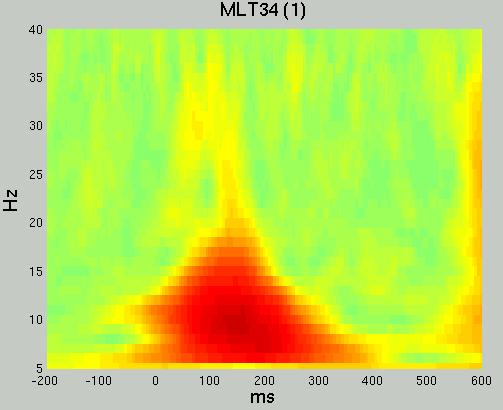
\includegraphics[width=60mm]{multimodal/figures/figure_32_14_R}
\caption{\em Phase-Locking Values for faces (left) and scrambled faces (right) for channel MLT34 \label{fig_32_14}}
\end{center}
\end{figure}

\subsection{2D Time-Frequency SPMs}

Analogous to Section~\ref{3DSPM}, we can also use Random Field Theory to correct for multiple statistical comparisons across the 2-dimensional time-frequency space.

* Type \verb!spm_eeg_convertmat2ana3Dtf! in the Matlab window, and select the \verb!t1_e_eeg.mat! file.

This will create time-frequency images for each trial of the two types, with dimensions 161x36x1, as for the example shown in Figure~\ref{fig_32_15} from pressing "Display: images" on the main SPM window.

\begin{figure}
\begin{center}
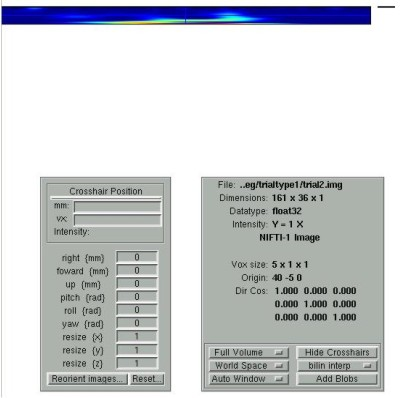
\includegraphics[width=100mm]{multimodal/figures/figure_32_15}
\caption{\em  3D image for trial 2 of t1-e-eeg.mat. The left section is through time (x) and frequency (y) (the right image is an y-z section, though there is only one value in z, i.e, it is really a 2D image).\label{fig_32_15}}
\end{center}
\end{figure}

As in Section~\ref{3DSPM}, we then take these images into an unpaired t-test across trials to compare faces versus scrambled faces. We can then use classical SPM to identify times and frequencies in which a reliable difference occurs, correcting across the multiple comparisons entailed (Kilner et al, 2005).

* First create a new directory, eg. mkdir TFstatsPow.

* Then press the "specify 2nd level" button,  select "two-sample t-test" (unpaired t-test), and define the images for "group 1" as all those in the subdirectory "trialtype1" (using right mouse, and "select all") and the images for "group 2" as all those in the subdirectory "trialtype2". Finally, specify the new TFstatsPow directory as the output directory, and press "run". (Note that this will be faster if you saved and could load an SPM job file from Section~\ref{3DSPM}).

This will produce the design matrix for a two-sample t-test.

* The press "Estimate", and when it has finished, press "Results" and define a new T-contrast as [1 -1]. Keep the default contrast options, but threshold at $p<.05$ FWE corrected for the whole "image". Then press "whole brain", and the Graphics window should now look like that in Figure~\ref{fig_32_16} (ignore the glass brain MIP).


\begin{figure}
\begin{center}
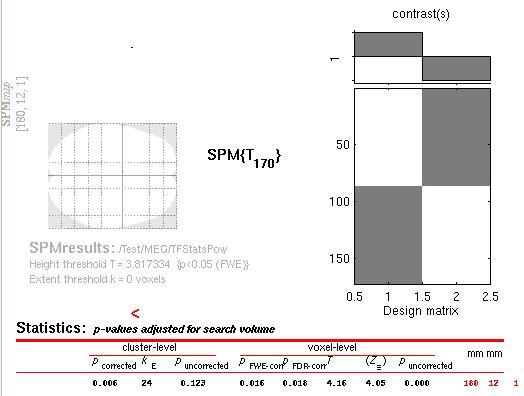
\includegraphics[width=100mm]{multimodal/figures/figure_32_16}
\caption{\em  2D time-frequency SPM{T} at $p<.001$ uncorrected for the power difference between face and scrambled faces at Channel MLT34. Note that the brain outline in the MIP should be ignored. The x  coordinates refer to time in ms; the y coordinates refer to frequency in Hz (the z-coordinate is always 1).\label{fig_32_16}}
\end{center}
\end{figure}

This will list one "region" within the 2D time-frequency space in which faces produce greater power than scrambled faces, having corrected for multiple T-tests across pixels. This has a maximum of  [180 12 1], ie 12 Hz and 180ms post-stimulus.

If you repeat the above time-frequency analysis on the \verb!e_meg.mat! file, but this time keep every channel and answer 'yes' to the "average over channels?" question, and then repeat the above statistical analysis of power, you will notice that there is also a reliable decrease in induced high-frequency power (around 400ms and 35 Hz) for faces vs scrambled faces, which could also be source-localised.


\subsection{"Imaging" reconstruction of differential power}

In Section~\ref{3D} we localised the differential evoked potential difference in EEG data corresponding to the N170.  Here we will localise the total power of faces vs scrambled faces in a timewindow corresponding to that of the M170, ie including potential induced components (see Friston et al, 2000).

* Press the '3D source reconstruction' button, and press the "load" button at the top of the new window. Select the \verb!e_meg.mat! file and type a label (eg "M170") for this analysis.

* Press the 'MRI' button, select 3000 for the number of vertices in the mesh, and select the smri.img file within the sMRI sub-directory...

This will take some time while the MRI is segmented and binary images of the skull created (see Section~\ref{3D} for more details on these files)\footnote{Note that this procedure can be shortened in the batch script included here, by loading the normalisation parameters and binary masks from previous segmentations of the structural MRI.}.

The choice of the minimum of 3000 vertices in the cortical mesh is simply to reduce computation time (the actual number of vertices resulting will be 3004).

Note that the cortical mesh (and the distances within the mesh) are not created directly from the segmented MRI (like the skull and scalp meshes), but rather are determined from a template cortical mesh in MNI space via inverse spatial normalisation (Mattout et al, in press).

When meshing has finished, the field D.inv\{1\}.mesh field will be updated in matlab. Press "save" in top right of window to update the corresponding mat file on disk. The cortex (blue), inner skull (red) and scalp (orange) meshes will also be shown in the Graphics window.

* Press the 'Co-register' button, respond "no" to the 'Read Polhemus?' question, and then select the following files in response to each prompt (pressing "yes" to the 'Use headshape file' prompt):
\begin{verbatim}
  		MEG/Polhemus/meg_sens_loc.mat
   		MEG/Polhemus/meg_fids.mat
   		MEG/Polhemus/meg_hsf.mat   	
  		MEG/Polhemus/meg_sens_or.mat	
		sMRI/smri_fids.mat
\end{verbatim}
	(like in Section~\ref{3DSPM}, except now we also need to provide information about the orientation of each MEG sensor, as in the penultimate file here).

This stage coregisters the MEG sensor positions and orientations (in "MEG" space) with the structural MRI and solution mesh (in "MRI" space). This is done via an approximate matching of the fiducials in the two spaces, followed by a more accurate surface-matching routine that fits the head-shape function (in "MEG" space) to the scalp that was created in the previous meshing stage via segmentation of the MRI. The match will be shown in a window like that in Figure~\ref{fig_32_17}. (Note that the match of the MEG and MRI fiducials is poor because the MEG fiducials did not correspond exactly to the nasion and peri-aricular points (see footnote 3); this does not matter because the coregistration is dominated by the close fit of the digitized headshape to the scalp mesh).

\begin{figure}
\begin{center}
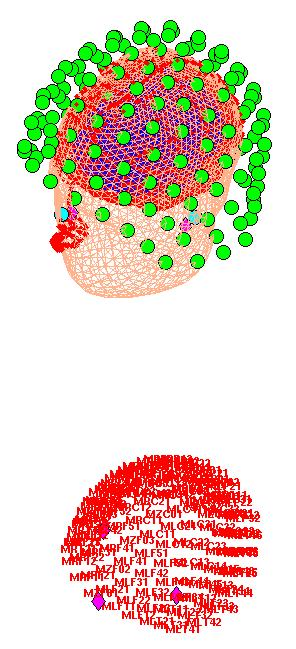
\includegraphics[width=70mm]{multimodal/figures/figure_32_17}
\caption{\em  Graphical output of registration of MEG and sMRI data, showing (upper panel) cortex (blue) and scalp (black) meshes, sensor locations (green), MRI and Polhemus fiducials (cyan/magneta), and headshape (red dots).\label{fig_32_17}}
\end{center}
\end{figure}

When coregistration has finished, the field D.inv\{1\}.datareg will be updated in matlab. Press "save" in top right of window to update the corresponding mat file on disk. Finally, a figure like that in Figure~\ref{fig_32_17} will also be produced, which you can rotate with the mouse (using the Rotate3D Matlab Menu option) to check all sensors.

* Press the 'Forward Model' button. This assumes the sensors lie on a single best-fitting sphere, which allows analytical computation of the forward model (lead field) that maps each "dipole" in the cortical mesh to each sensor, assuming that the orientation of the dipole at each vertex is normal to the surface of the mesh at that point. This stage uses BrainStorm functions~\footnote{Brainstorm is available from http://neuroimage.usc.edu/ResearchMEGEEGBrainStorm.html}. The Matlab window will output:
\begin{verbatim}
                Scalp best fitting sphere computed (in 11 iterations)
                Centre = [0.0001 -0.0218 0.0027] (Radius = 0.0774)
\end{verbatim}
* Press 'Invert.', select 'Classical', select 'yes' to 'All conditions or trials?', select 'MSP' (for Multiple Sparse Priors) for the type of inversion, "Standard" for the model (i.e, to use defaults; you can customise a number of options if you press Custom instead) (see Friston et al, in press-a, for more details about these parameters).

Press "save" to save the results. You can now explore the results via the 3D reconstruction window. If you type 165 into the box in the bottom right (corresponding to the time in ms) and press "mip", you should see an output like in Figure~\ref{fig_32_18}. This fit explains approx 87\% of the data.

Note the hot-spots in the fusiform. The timecourses come from the peak voxel. The red line shows the condition currently being shown (corresponding to the "Condition 1" toggle bar in the reconstruction window); the grey line(s) will show all other conditions. Condition 1 is faces; if you press the "condition 1" toggle, it will change to Condition 2 (scrambled faces), then press "mip" again and the display will update (note the colours of the lines have now reversed from before, with red now corresponding to scrambled faces).

If you toggle back to condition 1 and press "movie", you will see the changes in the source strengths over peristimulus time (from the limits 0 to 300ms currently chosen by default).

If you press "render" you can get a very neat graphical interface to explore the data (the buttons are fairly self-explanatory). However, we will concentrate on how one might perform statistics.


\begin{figure}
\begin{center}
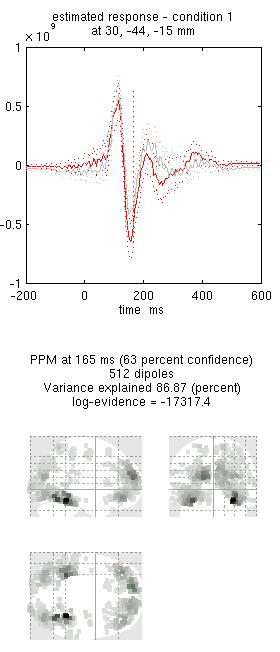
\includegraphics[width=100mm]{multimodal/figures/figure_32_18}
\caption{\em  Graphic output for MSP-estimated activity at 165ms for faces.\label{fig_32_18}}
\end{center}
\end{figure}

* Press the "Window" button in the reconstruction window, enter "150 200" as the timewindow of interest and "5 40" as the frequency band of interest. The Graphics window will show the mean activity for this time/frequency contrast (for faces alone, assuming the condition toggle is showing "condition 1").

* If you then press "Image", press "12" for the smoothing kernel, and SPM will write 3D Nifti images corresponding to the above contrast for each condition:
\begin{verbatim}
	w_e_meg_1_1.nii
	w_e_meg_1_2.nii
	sw_e_meg_1_1.nii
	sw_e_meg_1_2.nii
\end{verbatim}
Note that the first two images are unsmoothed (but normalised); the latter two are smoothed by a 12mm isotropic Gaussian kernel. The last number in the file name refers to the condition number; the penultimate number refers to the reconstruction number (ie the number in red in the reconstruction window, i.e, D.val, here 1).

The smoothed results for Condition 1 will also be displayed in the Graphics window, together with the normalised structural, as in Figure~\ref{fig_32_19}. Note that the solution image is in MNI (normalised) space, because the use of a canonical mesh provides us with a mapping between the cortex mesh in native space and the corresponding MNI space.

You can also of course view the image with the normal SPM "Display:image" option, and locate the coordinates of the "hotspots" in MNI space. Note that these images contain RMS (unsigned) source estimates (see Henson et al, 2007).

If you want to see where activity (in this time/freq contrast) is greater for faces and scrambled faces, you can use SPM's ImCalc to create a difference image of \verb!sw_e_meg_1_1.nii - sw_e_meg_1_2.nii! - you should see bilateral fusiform. For further discussion of localising a differential effect (as in Section~\ref{3D} with ERPs), vs taking the difference of two localisations, as here, see Henson et al (2007).

	

\begin{figure}
\begin{center}
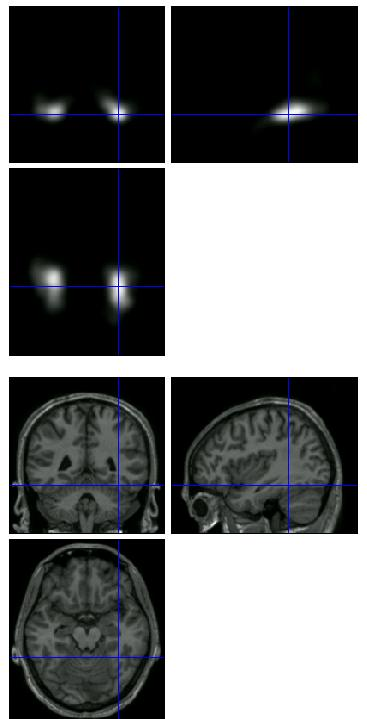
\includegraphics[width=100mm]{multimodal/figures/figure_32_19}
\caption{\em  Display of the smoothed 3D image of the MSP-estimated activity between 150-200ms in the frequency band 5-40Hz for faces, together with the normalised structural. Note large hotspots in bilateral fusiform.\label{fig_32_19}}
\end{center}
\end{figure}

You could also explore the other inversion options, like COH and MNM, which you will note give more superficial solutions (a known problem with standard minimum norm; see also Friston et al, in press-a). To do this quickly (without repeating the MRI segmentation, coregistration and forward modelling), press the "new" button in the reconstruction window, which by default will copy these parts from the previous reconstruction.


\section{fMRI analysis \label{fMRI}}

Only the main characteristics of the fMRI analysis are described below; for a more detailed demonstration of fMRI analysis, see Chapter 29.

Note that all the job files for each stage of preprocessing and analysis are also provided:
\begin{verbatim}
	fMRI/realign_job.mat
	fMRI/slicetime_job.mat
	fMRI/smooth_job.mat
	fMRI/stats_job.mat
\end{verbatim}
These can be loaded and run, though of course the location of the files and the output directory will need to be changed.

\subsection{Preprocessing the fMRI data}

* Toggle the modality from EEG to fMRI, and change directory to the fMRI subdirectory (either in Matlab, or via the "CD" option in the SPM "Utils" menu)

* Select 'Realign' from the 'Realign and Unwarp' menu, click on 'Data', and select 'New Session'. Double-click on the new Session branch, and click on the 'Images' button, click on the 'specify files' and select all 215 \verb!fM*.img! files in the Scan directory (using the right mouse to 'select all', assuming the filter is set to \verb!^f.*img!).

Realignment will produce a \verb!spm*.ps! postscript file in the current directory, which shows the estimated movement (like in Figure~\ref{fig_32_20}). Importantly, the resliced images will be output as rfM*.img files. A mean image will also be written:
\begin{verbatim}
		meanfMS02554-0003-000006.img
\end{verbatim}
as will the movement parameters in the text file:
\begin{verbatim}
		rp_fMS02554-0003-000006.txt
\end{verbatim}

.
\begin{figure}
\begin{center}
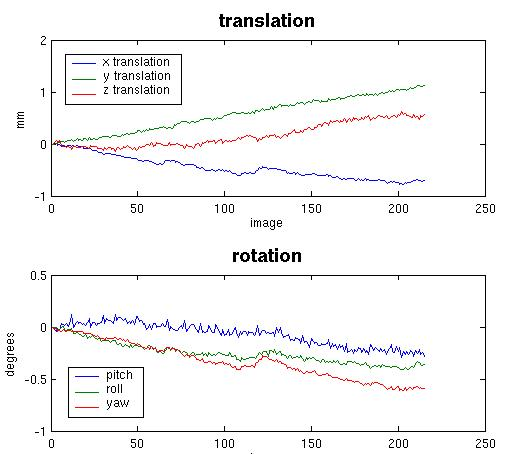
\includegraphics[width=100mm]{multimodal/figures/figure_32_20}
\caption{\em  Movement parameters from Realignment of the fMRI data. \label{fig_32_20}}
\end{center}
\end{figure}

* Press the 'slice-timing' button, select the functional images (filter set to \verb!^rf.*! to avoid the mean image), enter 2.88 as the TR, 2.88*31/32 as the TA, the slice-order as [1:32] (since the first slice in the file is the top slice, and this was the first slice acquired in the descending sequence), and the reference slice to 16. This will write out 215 images arfM*.img, in which the data have been interpolated to match the acquisition time of the middle slice (in space and time, given the sequential acquisition).

* Press the 'smooth' button and keep the default 10x10x10mm smoothing. This will produce 215 spatially-smoothed images sarfM*.img.

Note that we will not normalise these images, in order to compare them with the MEG and EEG source reconstructions, which are in the native MRI space.

\subsection{Statistical analysis of fMRI data}

* Load the onsets.mat file provided into the Matlab workspace

* Press the 'specify 1st-level' button, change the microtime onset from 1 to 8, select the 215 'sarfM*img' images, define two new conditions - condition 1 called "faces" with onsets set to onsets{1} and condition 2 called "scrambled faces" with onsets set to onsets{2} (all duration 0) - select the  \verb!rp_fMS02554-0003-000006.txt! file as 'Multiple Regressors' (to covary out some of the residual movement-related effects), and select the fMRI/Stats as the output directory (loading and editing the \verb!stats_job.mat! file provided will save a lot of time here!). Keep the rest of the parameters (e.g, use of a canonical HRF basis function) at their default settings.

This will produce a design matrix like that in Figure~\ref{fig_32_21}, which is stored in the file:
\begin{verbatim}
		fMRI/Stats/SPM.mat
\end{verbatim}

\begin{figure}
\begin{center}
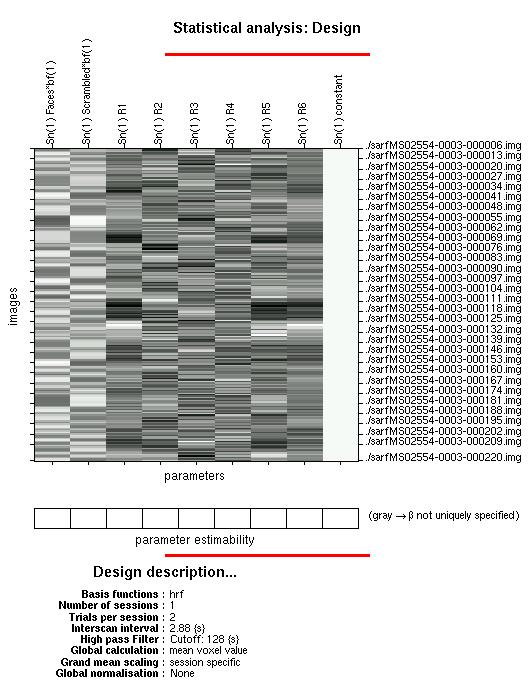
\includegraphics[width=100mm]{multimodal/figures/figure_32_21}
\caption{\em Design matrix for the fMRI analysis. \label{fig_32_21}}
\end{center}
\end{figure}

* Then estimate the parameters of the design matrix by pressing the 'Estimate' button and selecting the SPM.mat file

* Finally, to see the regions that respond differentially between faces and scrambled faces, press 'Results' and define a new F-contrast (called, e.g, 'Faces - Scrambled') by typing the contrast weights [1 -1].

This will identify regions in which the parameter estimate for the canonical HRF differs reliably between faces and scrambled faces. This could include regions that show both a "greater" relative response for faces, and regions that show a "greater" relative response for scrambled faces (such a two-tailed test is used because we do not know the precise relationship between haemodynamic changes measured by fMRI and the synchronous current changes measured by EEG/MEG).

If the resulting SPM{F} is thresholded at $p<.05$ FWE corrected, the resulting MIP and table of values should be like that in Figure ~\ref{fig_32_22}. Only two regions survive correction: right fusiform and orbitofrontal cortex (note coordinates refer to native MRI space; not MNI space). These can be displayed on the (attentuation-corrected) structural msmri.nii. They are a subset of the regions identified by the same contrast in a group of 18 subjects in Henson et al (2003). At a lower threshold (e.g, $p<.01$ uncorrected), one can see additional activation in left fusiform, as well as other regions.


\begin{figure}
\begin{center}
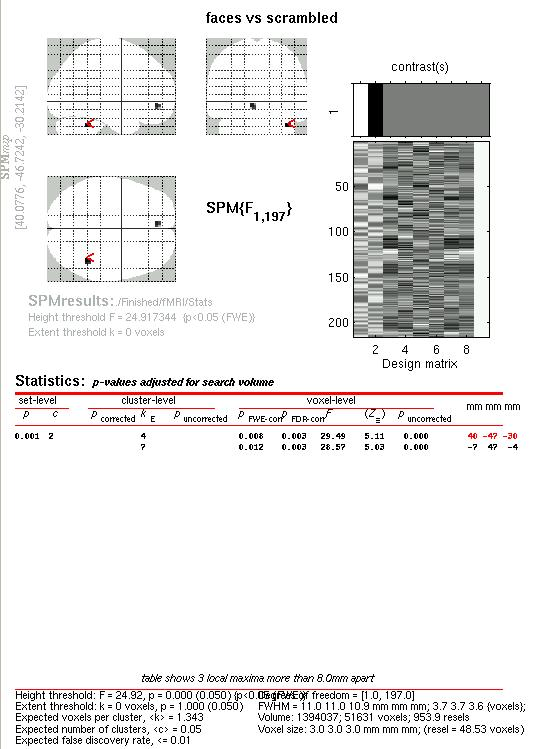
\includegraphics[width=100mm]{multimodal/figures/figure_32_22}
\caption{\em  SPM{F} for faces vs scrambled faces. Note that the coordinates are in the MRI native space (no normalisation performed) so bear a close, but not exact, relationship with MNI coordinates (affecting brain outline in MIP too).\label{fig_32_22}}
\end{center}
\end{figure}

There is some agreement between these fMRI effects and the localised EEG/MEG effects around the 170ms latency - eg in orbitofrontal and right fusiform - though of course the EEG dipoles were bilateral, and there were more extensive posterior occipitotemporal effects in the source-localised MEG data. Note of course that the fMRI data may include differences between faces and scrambled faces that occur at latencies other than the M170 (e.g, later), or differences in "induced" high-frequency M/EEG power that is not phase-locked to stimulus onset (Henson et al, 2005b).

One could use the unthresholded F-image as an additional continuous prior within the PEB L2-norm method offered by SPM5, or probably better, one could take a number of regions after thresholding the SPM{F}, and enter each as a separate prior on the PEB L2-norm method (this way, different regions can be up-weighted or down-weighted as a function of whether they are likely to be active during the critical timewindow being localised).



\section{References}

\noindent 1. Friston, K, Daunizeau, J, Kiebel, S, Phillips, C, Trujillo-Barreto, N, Henson, R, Flandin, G, Mattout, J (in press-a). Multiple sparse priors for the M/EEG inverse problem. Neuroimage. \\

\noindent 2. Friston, K, Carlton Chu, Janaina Mouro-Miranda, Oliver Hulme, Geraint Rees, Will Penny and John Ashburner (in press-b). Bayesian decoding of brain images. NeuroImage.\\

\noindent 3. Friston K, Henson R, Phillips C, and Mattout J. (2006). Bayesian estimation of evoked and induced responses. Human Brain Mapping, 27, 722-735.\\

\noindent 4. Henson, R, Goshen-Gottstein, Y, Ganel, T, Otten, L, Quayle, A. and Rugg, M. (2003). Electrophysiological and hemodynamic correlates of face perception, recognition and priming. Cerebral Cortex, 13, 793-805.\\

\noindent 5. Henson R, Mattout J, Friston K, Hassel S, Hillebrand A, Barnes G and Singh K. (2005a) Distributed source localisation of the M170 using multiple constraints. HBM05 Abstract.\\

\noindent 6. Henson R, Kiebel S, Kilner J, Friston K, Hillebrand A, Barnes G and Singh K. (2005b) Time-frequency SPMs for MEG data on face perception: Power changes and phase-locking. HBM05 Abstract.\\

\noindent 7. Henson, R.N. Mattout, J, Singh, K, Barnes, G, Hillebrand, A. and Friston, K.J. (2007). Population-level inferences for distributed MEG source localisation under multiple constraints: Application to face-evoked fields. Neuroimage, 38, 422-438.\\

\noindent 8. Josephs, O., Deichmann, R., Turner, R. (2000). Trajectory measurement andgeneralised reconstruction in rectilinear EPI. NeuroImage 11, S543.\\

\noindent 9. Kilner, J., Kiebel, S and Friston, K. J. (2005). Applications of random field theory to electrophysiology. Neuroscience Letters, 374:174-178.\\

\noindent 10. Kilner, J. and Penny. W. (2006). Robust Averaging for EEG/MEG. HBM06 Abstract.\\

\noindent 11. Kiebel S and Friston K (2004). Statistical Parametric Mapping for Event-Related Potentials II: A Hierarchical Temporal Model. NeuroImage, 22, 503-520.\\

\noindent 12. Kiebel, S.J., David, O. and Friston, K. J. (2006). Dynamic Causal Modelling of Evoked Responses in EEG/MEG with lead-field parameterization. NeuroImage, 30:1273-1284.\\

\noindent 13. Mattout J, Pelegrini-Issac M, Garnero L and Benali H. (2005a). Multivariate source prelocalization (MSP): use of functionally informed basis functions for better conditioning the MEG inverse problem. Neuroimage, 26, 356-73.\\

\noindent 14. Mattout, J, Phillips, C, Penny, W, Rugg, M and Friston, KJ (2005b). MEG source localisation under multiple constraints: an extended Bayesian framework. NeuroImage.\\

\noindent 15. Mattout, J., Henson, R N. and Friston, K.J. (in press). Canonical Source Reconstruction for MEG. Computational Intelligence and Neuroscience.\\

\noindent 16. Phillips, C. M.D. Rugg, M and Friston, K (2002). Systematic Regularization of Linear Inverse Solutions of the EEG Source Localisation Problem. NeuroImage, 17, 287-301.\\

\noindent 17. Spinelli, L, Gonzalez S, Lantz, G, Seeck, M and Michel, C. (2000). Electromagnetic inverse solutions in anatomically constrained spherical head models. Brain Topography, 13, 2.\\

